\documentclass[tikz, border=10pt]{standalone}
\usepackage{pgfplots}
\pgfplotsset{compat=1.18}

\begin{document}
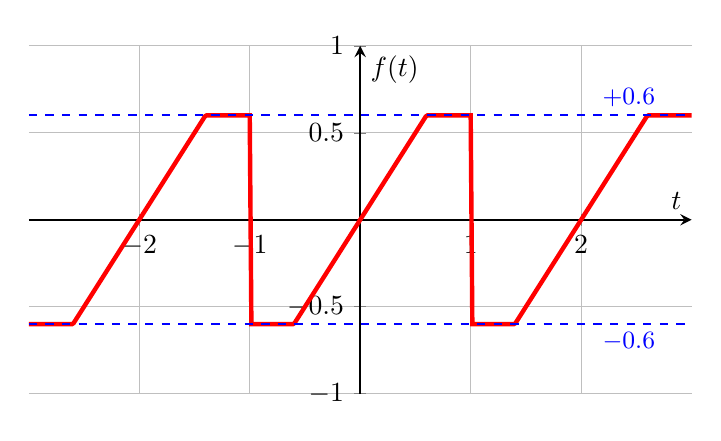
\begin{tikzpicture}
    \begin{axis}[
        width=10cm, height=6cm,
        axis lines=middle,
        xlabel={$t$}, ylabel={$f(t)$},
        ymin=-1.0, ymax=1.0,
        xmin=-3, xmax=3,
        xtick={-2, -1, 0, 1, 2},
        grid=both,
        samples=400,
        domain=-3:3,
        thick
    ]
        % Sawtooth clipped at +/- 0.6
        % Sawtooth: t - 2*floor((t+1)/2)
        \addplot[red, ultra thick] {max(-0.6, min(0.6, x - 2*floor((x+1)/2)))};
        
        \draw[dashed, blue] (axis cs:-3, 0.6) -- (axis cs:3, 0.6);
        \draw[dashed, blue] (axis cs:-3, -0.6) -- (axis cs:3, -0.6);
        \node[blue, right] at (axis cs:2.1, 0.7) {\small $+0.6$};
        \node[blue, right] at (axis cs:2.1, -0.7) {\small $-0.6$};
    \end{axis}
\end{tikzpicture}
\end{document}
